
\chapter{Point cloud based methods}
\label{ch:point_cloud_based}

Reconstructing surfaces from point clouds is a lively branch in computational geometry.
As discussed when summarizing the state of the art, \cf chapter \ref{ch:state_of_the_art}, several well-working methods have been developed to convert a set of points into a polyhedral surface, \ie triangle meshes in most cases.
One possible explanation for this richness in algorithms is that point clouds are heavily used for their simplicity when digitizing real-world objects, \eg by scanning their surface with lasers or depth-sensing cameras.

Some algorithms temporarily create intermediate representations, \eg Voronoi diagrams and medial axes, like the cocone \cite{cocone, tight_cocone, robust_cocone} and crust \cite{crust, power_crust} family, or functional ones, like the MLS \cite{mls}, RBF \cite{rbf} or signed distance functions \cite{sdf_surface_reconstruction} approaches.
Thus, some of these algorithms have other uses as well beside surface reconstruction.
Other methods create surface triangles directly, mostly by growing a region on the sampled surface.
They are typically faster but more susceptible to noisy input, \eg BPA and G2S.
Nevertheless, this collection of algorithms should also be available for reconstructing surfaces from the VML's data model.

In the previous chapter \ref{ch:tri_dexel}, the tri-dexel based surface reconstruction approach relied on a raycast to sample the VML's regular grid into dexels.
This raycast may just as well be used to sample other data structures as well.
In its simplest form, by only collecting the surface hits, a point cloud is obtained.
This point cloud may then be used as input to probably all point cloud based surface reconstruction algorithms, including the ones mentioned above.

Compared with the other two implementation chapters \ref{ch:direct_intersection} and \ref{ch:tri_dexel}, this chapter resembles more an additional idea than a serious implementation.
The reason for this is that reconstructing a surface, especially with features, turned out to be much harder from a point cloud than from semantically richer data structures such as a tri-dexel image.
Currently, the tri-dexel approach is the preferred reconstruction approach inside the VML.
However, giving the ability to export a point cloud opens up another huge world of research work and algorithms, and is therefore shortly discussed in this chapter.


\section{Concept}
\label{sec:point_cloud_concept}

Using any kind of point cloud based algorithm for surface reconstruction from the VML's data model, boils down to two steps.
Firstly, a point cloud has to be created from the VML's data model.
This step is very similar and even simpler than the creation of the dexel image discussed in the previous chapter \ref{ch:tri_dexel}.
The same raycasting technique, with all its error correcting and robustness enhancing code, will be used to sample surface intersections on the VML's data model.
The resolution of the raycasting grid for each of the three axis-aligned casts is again supplied by the user, again providing a good parameter for steering quality and computational demands.
Figure \ref{fig:cylinder_head_point_cloud} shows a point cloud created from the cylinder\_head scene using a raycast with resolution 200.
%
\begin{figure}
	\centering
	\begin{subfigure}[t]{0.49\textwidth}
		\centering
		\includegraphics[width=\textwidth]{images/cylinder_head_point_cloud}
		\caption{cylinder\_head}
		\label{fig:cylinder_head_point_cloud_}
	\end{subfigure}
	\begin{subfigure}[t]{0.49\textwidth}
		\centering
		\includegraphics[width=\textwidth]{images/cylinder_head_point_cloud_fins}
		\caption{fins}
		\label{fig:cylinder_head_point_cloud_fins}
	\end{subfigure}
	\caption{
		Point cloud created by raycasting the cylinder\_head scene using three axis-aligned raycasts along the coordinate system's axes with a resolution of 200.
	}
	\label{fig:cylinder_head_point_cloud}
\end{figure}
%
Secondly, after the point cloud has been created, a surface reconstruction algorithm is run on it.

Regarding its quality, a point cloud sampled from the VML's regular grid using a uniform, axis-aligned raycast has a few properties:
\begin{itemize}
	\item
	All surface points, excluding numeric errors, are usually perfect samples, lying directly on the workpiece's surface.
	There is neither noise on the surface nor are there irrelevant inner or outer points.
	\item
	Each surface sample provides a perfect surface normal.
	\item
	The regularity of the raycaster guarantees a minimum and maximum density of the cloud, which may be derived from the ray distances along each axis.
\end{itemize}

Despite these quality guarantees, a point cloud is still less rich in semantics when compared with a tri-dexel image.
The most prominent differences and commonalities are:
\begin{itemize}
	\item
	Point clouds only store surface information, whereas a tri-dexel image also holds volumetric information, \ie the dexel segments and point occupancy of the tri-dexel grid.
	\item
	Although a sufficient density is necessary, point clouds do not profit from the regular and uniform sampling.
	This property is fundamental for the tri-dexel approach, as it enables the construction of the regular tri-dexel grid and breaks down the problem of triangulation.
	\item
	The regularization of the tri-dexel cells provides a good way of detecting feature-rich regions which should be resampled with increased density.
	Such regions are harder to find with a point cloud, although local point distance and normal variance might give good hints.
	\item
	Although no regularization step is needed for small peculiarities of the cloud, it depends solely on the used reconstruction algorithm whether such information can be extracted or is left unused.
	Regarding the tri-dexel approach presented in chapter \ref{ch:tri_dexel}, such behavior is well-defined by either regularizing, \ie dropping, or slicing a cell with small features.
	\item
	In both cases, features which are not discovered by the raycaster are not present in the built data structures.
	Subsequent algorithms have to implement some kind of feature reconstruction.
	\item
	Point clouds are simpler data structures and easier to exchange with other 3D software.
	\item
	Point clouds have a substantially smaller memory footprint than tri-dexel images.
\end{itemize}


\section{Implementation}
\label{sec:point_cloud_implementation}

Reusing the axis-aligned raycast from section \ref{sec:tri_dexel_raycast}, all reported surface intersections are just accumulated into a set of points.
Afterwards, any kind of surface reconstruction algorithm may used to proceed.

\subsection{Point cloud creation}
\label{sec:point_cloud_creation}

Algorithm \ref{alg:point_cloud_based} shows the basic routine used to obtain a point cloud and call a subsequent reconstruction algorithm.
%
\begin{algorithm}
	\centering
	\begin{algorithmic}[1]
		\Function{PointCloudBased}{$\var{grid}, \var{resolution}$}
			\State $\var{res} = \Call{UniformResolution}{\var{grid}.\var{aabb}, \var{resolution}}$
			\State $\var{cloud} = \varnothing$
			\State $\Call{AxisParallelRaycast}{\var{grid}, \var{grid}.\var{aabb}, \var{res},\hfill\break
				\hspace*{\dimexpr\algorithmicindent*2}(\var{\_}, \var{\_}, \var{\_}, \var{v}, \var{n}) \rightarrow \var{cloud}.\var{add}((\var{v}, \var{n}))}$
			\State \Return $\Call{ReconstructFromPointCloud}{\var{cloud}}$
		\EndFunction
	\end{algorithmic}
	\caption{
		Abstract workflow of the surface reconstruction using an arbitrary point cloud reconstruction algorithm \textproc{ReconstructFromPointCloud}.
	}
	\label{alg:point_cloud_based}
\end{algorithm}
%
Using the \textproc{UniformResolution} function, the algorithm starts off by computing an appropriate raycasting resolution \var{res} for all three axes, based on the \var{resolution} parameter passed by the user.
This step is also done before the tri-dexel raycast, but with an increased bounding box, \cf algorithm \ref{alg:tri_dexel}.
For the details of \textproc{UniformResolution} \cf section \ref{sec:tri_dexel_implementation}.
Afterwards, an empty set of points, \var{cloud}, is created, which will accumulate all surface points emitted by the raycaster.
Afterwards, the raycast is launched with the calculated resolution and the grid's bounding box.
The closure passed to the raycasting subroutine \textproc{AxisParallelRaycast} is called at every surface hit with a list of arguments.
From these arguments only the last two, the intersection point \var{v} and the corresponding surface normal \var{n}, are relevant.
These two are added as tuple to the current point cloud \var{cloud}.
After the raycast has finished, a point cloud based surface reconstruction algorithm is run, indicated by the call to \textproc{ReconstructFromPointCloud}.

\subsection{Surface reconstruction}
\label{sec:point_cloud_reconstruction}

A few examples of algorithms for surface reconstruction from point clouds are given in the following:

\begin{description}
	\item[Ball pivoting algorithm] \hfill \\
	The ball pivoting algorithm (BPA) is a region growing algorithm.
	As the name suggests, it places a ball, \ie sphere, at the outside of the point cloud, touching three points, creating a seed triangle.
	From this seed triangle, the ball is pivoted over each edge of the triangle until it touches another point, creating a new triangle with new edges to roll over.
	If no point is found during pivoting, the edge is left as a boundary.
	The front of edges is rolled over repeatedly until no more edges are available.
	If all pivots where successful, a closed, manifold and oriented mesh has been created.
	The BPA requires a user supplied ball size, which steers the capability of rolling into finer features and the danger of creating holes or falling into the point cloud.
	A highly tuned version of the BPA with elements of the G2S algorithm is already utilized by the VML for its swept volume computation \cite{bpa_vml}.
	An implementation of the BPA is available in CGAL \cite{cgal_bpa}.
	MeshLab also offers a BPA version, parameterizable via its GUI.

	\item[$\alpha$-shape] \hfill \\
	The $\alpha$-shape was one of the first tries to define a \enquote{shape} for a set of finite points \cite{alpha_shape}.
	The $\alpha$-shape of a 3-dimensional point cloud is a set of triangles, where each triangle has at least one empty circumsphere with radius $\alpha$.
	It is quite similar to the BPA, but formulated statically, as no ball is rolled along the surface.
	The $\alpha$-shape therefore also contains triangles within the point cloud, which would not be discovered by the BPA if the ball never rolls \enquote{inside} the point cloud, \ie sufficient density is given.
	If $\alpha$ becomes $\infty$, the $\alpha$-shape becomes the convex hull of the point cloud.
	The empty circumsphere criterion further guarantees the triangulation to be Delaunay, \ie the $\alpha$-shape is a subset of the 3-dimensional Delaunay triangulation.
	An implementation of an $\alpha$-shape constructing algorithm is found in \eg the CGAL \cite{cgal_3d_alpha_shapes}, VTK \cite{vtk}, QHull \cite{qhull} or PCL \cite{pcl} library.
	MeshLab provides user-friendly access the QHull version of the algorithm via a GUI.

	\item[Poisson] \hfill \\
	Poisson surface reconstruction is based on implicit functions \cite{poisson}.
	The goal is to compute a so-called indicator function $\chi$, which yields 1 for positions inside the workpiece and 0 for positions outside.
	When moving into the workpiece from outside, the values of $\chi$ change from 0 to 1 around the surface.
	The indicator function $\chi$, specifically its gradient $\nabla\chi$, is strongly related to the normals of the input point set, a vector field $V$.
	Therefore, the problem becomes finding a function $\chi$ whose gradient $\nabla\chi$ best approximates $V$, the normals of the point cloud, \ie $\min_\chi |\nabla\chi - V|$.
	This problem is then transformed into a standard Poisson problem and further detailed \cite{poisson}.
	For the computation of these functions the problem space is partitioned using an octree, whose depth provides the main variable to balance memory/computational demands and reconstruction quality.
	The reconstruction of a surface is finally done by extracting an iso surface of $\chi$.
	Implementations of Poisson surface reconstruction are found in \eg the CGAL \cite{cgal_poisson}, VTK \cite{vtk_poisson} and PCL \cite{pcl} library.
	MeshLab also integrates a Poisson implementation into its GUI.
\end{description}


\section{Results}
\label{sec:point_cloud_results}

The point cloud creation and the subsequent reconstruction using the few algorithms discussed in \cite{sec:point_cloud_creation} have been benchmarked for the test scenes described in section \ref{sec:test_scenes}.
Analogously to the tri-dexel benchmarks, the resolutions 50, 100, 200 and 400 have been used for the raycaster creating the point clouds.
Table \ref{tbl:point_cloud_results} contains the runtime and output size of the created point clouds.
%
\begin{table}
	\begin{tabular}{l|rr|rr|rr|rr}
		resolution     & \multicolumn{2}{c}{50} & \multicolumn{2}{c}{100} & \multicolumn{2}{c}{200} & \multicolumn{2}{c}{400} \\
		scene          & p\sub{out} & time & p\sub{out} & time & p\sub{out} & time & p\sub{out} & time \\
		\midrule
		cube2          & \SI{14}{\kilo\nothing} & \SI{  3}{\milli\second} & \SI{56}{\kilo\nothing} & \SI{ 12}{\milli\second} & \SI{226}{\kilo\nothing} & \SI{  47}{\milli\second} & \SI{907}{\kilo\nothing} & \SI{ 187}{\milli\second} \\
		cylinders\_d   & \SI{ 7}{\kilo\nothing} & \SI{  5}{\milli\second} & \SI{27}{\kilo\nothing} & \SI{ 17}{\milli\second} & \SI{108}{\kilo\nothing} & \SI{  63}{\milli\second} & \SI{436}{\kilo\nothing} & \SI{ 247}{\milli\second} \\
		cylinders      & \SI{ 7}{\kilo\nothing} & \SI{  3}{\milli\second} & \SI{26}{\kilo\nothing} & \SI{ 11}{\milli\second} & \SI{107}{\kilo\nothing} & \SI{  41}{\milli\second} & \SI{433}{\kilo\nothing} & \SI{ 161}{\milli\second} \\
		cylinder\_head & \SI{15}{\kilo\nothing} & \SI{  7}{\milli\second} & \SI{60}{\kilo\nothing} & \SI{ 23}{\milli\second} & \SI{242}{\kilo\nothing} & \SI{  86}{\milli\second} & \SI{976}{\kilo\nothing} & \SI{ 335}{\milli\second} \\
		impeller       & \SI{11}{\kilo\nothing} & \SI{ 99}{\milli\second} & \SI{46}{\kilo\nothing} & \SI{353}{\milli\second} & \SI{184}{\kilo\nothing} & \SI{1118}{\milli\second} & \SI{744}{\kilo\nothing} & \SI{3813}{\milli\second} \\
		impeller\_2    & \SI{ 9}{\kilo\nothing} & \SI{ 54}{\milli\second} & \SI{38}{\kilo\nothing} & \SI{193}{\milli\second} & \SI{155}{\kilo\nothing} & \SI{ 600}{\milli\second} & \SI{625}{\kilo\nothing} & \SI{2037}{\milli\second} \\
		turbine        & \SI{ 7}{\kilo\nothing} & \SI{165}{\milli\second} & \SI{31}{\kilo\nothing} & \SI{650}{\milli\second} & \SI{132}{\kilo\nothing} & \SI{2509}{\milli\second} & \SI{532}{\kilo\nothing} & \SI{9610}{\milli\second} \\
	\end{tabular}
	\caption{
		Test results for the point cloud creation.
		Benchmarks were run on a machine utilizing an Intel Core i7-3770 at \SI{3.4}{\giga\hertz} with \SI{16}{\gibi\byte} RAM.
		Runtime is averaged over 10 runs.
	}
	\label{tbl:point_cloud_results}
\end{table}
%
Three trends, similarly to the results of the tri-dexel reconstruction in table \ref{tbl:tri_dexel_results}, are also observable here.
Firstly, the number of created points p\sub{out} for a given resolution is again similar for all scenes.
Secondly, p\sub{out} increases quadratically with the resolution.
Thirdly, also the runtime increases quadratically with the resolution.
The reasons is the asymptotic complexity of $\mathcal{O}(n^2)$ of the raycaster, which is discussed in more detail in section \ref{sec:tri_dexel_results}.
Furthermore, the dependency of the runtime on the scene's complexity as well as parallelization, CPU and memory consumption is also discussed there.

Concerning subsequent surface reconstruction algorithms, table \ref{tbl:bpa_results} contains the mesh sizes and timings for the VML's BPA implementation.
The ball's radius is derived from the raycasting resolution and set to 1.5 times the diameter of a cell of the sampling grid created by 3 axis aligned raycasts.
%
\begin{table}
	\begin{tabular}{l|rrr|rrr}
		resolution     & \multicolumn{3}{c}{50} & \multicolumn{3}{c}{100} \\
		scene          & p\sub{in} & t\sub{out} & time & p\sub{in} & t\sub{out} & time \\
		\midrule
		cube2          & \SI{14}{\kilo\nothing}& \SI{27}{\kilo\nothing} & \SI{53}{\milli\second} & \SI{56}{\kilo\nothing} & \SI{111}{\kilo\nothing} & \SI{222}{\milli\second} \\
		cylinders\_d   & \SI{ 7}{\kilo\nothing}& \SI{13}{\kilo\nothing} & \SI{22}{\milli\second} & \SI{27}{\kilo\nothing} & \SI{ 53}{\kilo\nothing} & \SI{ 95}{\milli\second} \\
		cylinders      & \SI{ 7}{\kilo\nothing}& \SI{13}{\kilo\nothing} & \SI{22}{\milli\second} & \SI{26}{\kilo\nothing} & \SI{ 53}{\kilo\nothing} & \SI{ 94}{\milli\second} \\
		cylinder\_head & \SI{15}{\kilo\nothing}& \SI{27}{\kilo\nothing} & \SI{60}{\milli\second} & \SI{60}{\kilo\nothing} & \SI{110}{\kilo\nothing} & \SI{223}{\milli\second} \\
		impeller       & \SI{11}{\kilo\nothing}& \SI{20}{\kilo\nothing} & \SI{48}{\milli\second} & \SI{46}{\kilo\nothing} & \SI{ 91}{\kilo\nothing} & \SI{200}{\milli\second} \\
		impeller\_2    & \SI{ 9}{\kilo\nothing}& \SI{17}{\kilo\nothing} & \SI{36}{\milli\second} & \SI{38}{\kilo\nothing} & \SI{ 76}{\kilo\nothing} & \SI{161}{\milli\second} \\
		turbine        & \SI{ 7}{\kilo\nothing}& \SI{ 9}{\kilo\nothing} & \SI{20}{\milli\second} & \SI{31}{\kilo\nothing} & \SI{ 53}{\kilo\nothing} & \SI{142}{\milli\second} \\
	\end{tabular}
	\bigskip\\
	\begin{tabular}{l|rrr|rrr}
		resolution     & \multicolumn{3}{c}{200} & \multicolumn{3}{c}{400} \\
		scene          & p\sub{in} & t\sub{out} & time & p\sub{in} & t\sub{out} & time \\
		\midrule
		cube2          & \SI{226}{\kilo\nothing}& \SI{449}{\kilo\nothing} & \SI{1022}{\milli\second} & \SI{907}{\kilo\nothing}& \SI{1807}{\kilo\nothing} & \SI{5106}{\milli\second} \\
		cylinders\_d   & \SI{108}{\kilo\nothing}& \SI{217}{\kilo\nothing} & \SI{ 442}{\milli\second} & \SI{436}{\kilo\nothing}& \SI{ 871}{\kilo\nothing} & \SI{1999}{\milli\second} \\
		cylinders      & \SI{107}{\kilo\nothing}& \SI{215}{\kilo\nothing} & \SI{ 421}{\milli\second} & \SI{433}{\kilo\nothing}& \SI{ 865}{\kilo\nothing} & \SI{1902}{\milli\second} \\
		cylinder\_head & \SI{242}{\kilo\nothing}& \SI{454}{\kilo\nothing} & \SI{ 946}{\milli\second} & \SI{976}{\kilo\nothing}& \SI{1850}{\kilo\nothing} & \SI{4263}{\milli\second} \\
		impeller       & \SI{184}{\kilo\nothing}& \SI{368}{\kilo\nothing} & \SI{ 859}{\milli\second} & \SI{744}{\kilo\nothing}& \SI{1485}{\kilo\nothing} & \SI{3710}{\milli\second} \\
		impeller\_2    & \SI{155}{\kilo\nothing}& \SI{309}{\kilo\nothing} & \SI{ 695}{\milli\second} & \SI{625}{\kilo\nothing}& \SI{1248}{\kilo\nothing} & \SI{3135}{\milli\second} \\
		turbine        & \SI{132}{\kilo\nothing}& \SI{246}{\kilo\nothing} & \SI{ 613}{\milli\second} & \SI{532}{\kilo\nothing}& \SI{1049}{\kilo\nothing} & \SI{2222}{\milli\second} \\
	\end{tabular}
	\caption{
		Test results surface reconstruction using the VML's internal BPA implementation excluding the time required to generate the point cloud, \cf table \ref{tbl:point_cloud_results}.
		Benchmarks were run on a machine utilizing an Intel Core i7-3770 at \SI{3.4}{\giga\hertz} with \SI{16}{\gibi\byte} RAM.
		Runtime is averaged over 10 runs.
	}
	\label{tbl:bpa_results}
\end{table}
%
Compared with the tri-dexel results in table \ref{tbl:tri_dexel_results}, the BPA outputs less than a half as much triangles.
This is due to the additional feature reconstruction and triangle fans created inside each cell by the tri-dexel approach.
As the BPA only operates on the vertices of the point cloud, it cannot create any further vertices.

Another consequence of this behavior is a correlation of the number of input points, \cf table \ref{tbl:point_cloud_results}, and the number of outputted triangles, \cf table \ref{tbl:bpa_results}.
For each point of the input roughly two triangles are created.
This ratio is smaller at lower resolutions as more features/points are skipped by the ball's size, but, with increasing density, almost all points are used by the BPA and this ratio approaches two.
An explanation for this ratio is given in figure \ref{fig:bpa_point_triangle_ratio}.
%
\begin{figure}
	\centering
	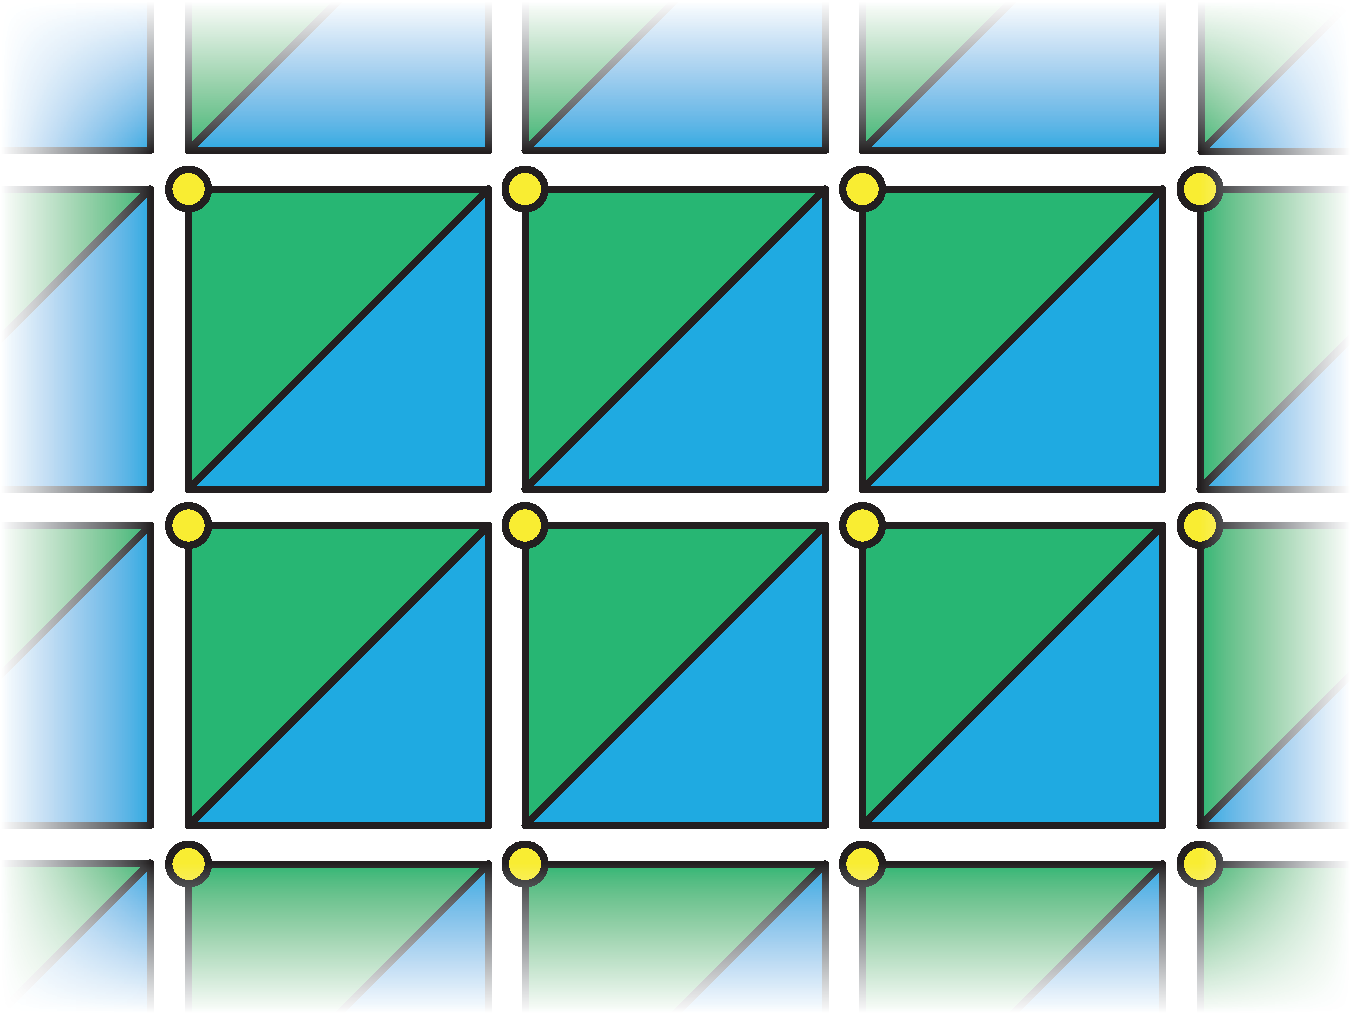
\includegraphics[width=0.6\textwidth]{images/bpa_point_triangle_ratio}
	\caption{
		Explanation for the ratio between mesh size and point cloud size approaching 2.
		If the surface of an object and the corresponding points and triangles are completely unwrapped into a plane, each surface point may be associated with exactly two triangle.
	}
	\label{fig:bpa_point_triangle_ratio}
\end{figure}
%
This correlation now allows to calculate an approximation for the input raycasting resolution given a number of output triangles, which becomes handy if a triangle budget is specified for the output mesh.

The BPA timings in table \ref{tbl:bpa_results}, especially at higher resolutions, further show that the algorithm's runtime is strongly related to the number of points of the cloud.
For each \SI{1}{\kilo\nothing} points, the BPA requires roughly \SI{4}{\milli\second} runtime, emitting \SI{2}{\kilo\nothing} triangles.
At lower resolutions, the parallelization overhead becomes visible, which is not as straight-forward as for the embarrassingly parallel tri-dexel or direct intersection, \cf the corresponding paper \cite{bpa_vml}.

